\chapter{Write Away 9}

\begin{figure}[H]
    \centering
    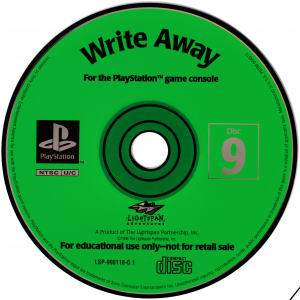
\includegraphics[width=\textwidth/2]{./Games/WriteAway/Images/WriteAway9CD.png}
    \caption{Write Away 9 CD}
\end{figure}

The ninth of the ten Write Away games published and released by The Lightspan Partnership for the PlayStation 1.

Write Away 9 features nine video programs, including an introduction video, seven story videos, and a conclusion video:

\begin{itemize}
    \item Write Away Episode Nine Introduction
    \item The MacMillain Mixup by Torri Newman
    \item A Dragon by Erikalyn Bassaraba
    \item Friendship by Candace Taylor
    \item The Pirates from Cinnabar by R.
          Peckham, S.
          Sengupta, H.
          Kramek and T.
          LaJoie
    \item Journey to the Centre of the Earth by Tranette Brunson
    \item My Husky Dog My Good Cat by Ami Benitez and Shaun Seumptewa
    \item The Lost Boy by Michael Singletary
    \item Write Away Conclusion
\end{itemize}

\clearpage
\newpage

JOE
SABRINA
SCOUT
JENNIFER
PAUL

\section{Transcriptions}

\subsection{The MacMillain Mixup by Torri Newman}

SCOUT:
Have you ever wondered what it would be like to travel back in time?
To the time of kings and queens and knights?
Well, you can't really travel back in time, but you can go anywhere you want, any time you want, simply by putting yourself in your very own story.
And that's just what our next author did.
Torri Newman from in Mesa, Arizona put herself into her own narrative entitled The MacMillion Mix-Up.

TORRI:
The story I'm about to tell you may sound a little bit strange, but it really happened to me.
It all began one dark night.

TORRI (VOICE OVER):
I was reading when I fell asleep.
I awoke to a loud crash.
A huge vase had fallen and broken into a million pieces.

TORRI:
How did that happen, and how did it get in my room?
Where am I, and where's the sign on my door that reads 'Torri's room, keep out'?
How did I get here?

TORRI (VOICE OVER):
Suddenly, a big fluffy dog ran into the room and jumped on me.
Then a strange looking man in odd clothes came in and said\dots

RALPH:
James, James, get down!
Oh, I am so sorry mistress Victoria, it's just that he got out of my grip.
Why, you look so pale - like a ghost.

TORRI:
W-who are you, and where am I?

RALPH:
Oh dear, you must be sick not to remember who I am.
I've lived at the MacMillion Castle ever since you were a little girl.
I-I'm Ralph, your servant.
Basically the one who has taken care of your whole life.

TORRI:
And, where did you say I was, and, what's the date?

RALPH:
Oh dear dear dear!
You are in your mother and father's castle, and it is April 13, 1126.

TORRI:
1126!
Ooh!
*faints*

RALPH:
Oh my, my my my.

TORRI (VOICE OVER):
When I woke up, everyone was standing over me with a woman saying,

DREAM MOTHER:
Oh, my baby.
My baby.
Are you all right?

TORRI:
Who are you?

DREAM MOTHER:
Oh, I'm your mother, your mother, your mother.

TORRI:
I'm outta here!

TORRI (VOICE OVER):
I ran and ran until I reached a dead end.
I turned around, gasping for air, they were running down the hall after me.
They were getting closer and closer, when I felt a rush of air and\dots

MOM:
TORRI, this is the last time I call you to dinner before I give it to the dog!

TORRI:
I'm in my own room, in my own bed!
Woo!
And to this day, I still can't figure out what happened.
All I know is, no more peanut butter and pickle sandwiches before bedtime.

\subsection{A Dragon by Erikalyn Bassaraba}

SABRINA:
And they lived happily ever after.
A typical ending for a fairy tale, right?
Well, I have a new fairy tale.
It has many elements of a fairy tale, like magic and dragons, but with a modern story's unusual twist.
It was written by Erikalyn Basaraba of Henry School in Tucson, Arizona.
Her new tale is called 'A Dragon'.

NARRATOR (SABRINA):
Once upon a time, long, long ago, there lived a baby dragon named Mikey.
He was a nice, helpful dragon.
One day, he met a strange lady who needed his help.

MAGICAL LADY:
Hello, little dragon.

MIKEY:
Who are you?

MAGICAL LADY:
I am the lady of magic.
I make things appear and disappear.
I can do all sorts of magical things!

MIKEY:
Duh, I don't believe that you have magic.
Prove it to me.

NARRATOR (SABRINA):
So that the little dragon would believe, the magical lady waved her hands across the sky, and lightning flashed, and beautiful mountains came to be.

MAGICAL LADY:
Now do you believe?

MIKEY:
I believe you.

MAGICAL LADY:
Good, for I need your help.
Oh, I've lost all my gold.
A mean little troll threw it into the ocean, and I cannot touch salt water.
If you get it for me, I will grant you one wish.

MIKEY:
But I'm a dragon.
I can't swim.
I can only fly.

MAGICAL LADY:
Hmm, ah - I've got it!
Close your eyes.

NARRATOR (SABRINA):
And with a wave of her hands, the magical lady turned Mikey the dragon into a mermaid.

MIKEY:
Now, to find the gold.

NARRATOR (SABRINA):
The mermaid swam deep down and found the gold, then she swam back up and gave the gold to the lady.

MIKEY:
I love being a mermaid.
My wish is to stay this way forever.
I shall be called Michelle.

MAGICAL LADY:
And I will give you a new friend.
Merman, come and meet your new friend.

MAX:
Hi, I'm Max the merman.
Let's swim!

NARRATOR (SABRINA):
They both lived happily ever after, but as for the magical lady, she took her gold to Las Vegas and lost it all in the slot machines.

MAGICAL LADY:
Jackpot!
Jackpot!
Jackpot!
Lemon?
Oh, I've lot all my gold!

ELVIS:
That's the way it goes in Vegas, baby.

MAGICAL LADY:
Ah, the king?

ELVIS:
Viva Las Vegas!

\subsection{Friendship by Candace Taylor}

JENNIFER:
We've had a lot of stories about people whom the authors know.
Our next writer lets us know about a special person in her life, but she does so in a different way.
She uses my favorite form of writing - poetry.
Candace Taylor from Conti School in New Jersey lets us see how important a friend is in her poem Friendship.

GIRL 1:
I have a friend who likes to talk.

GIRL 2:
And I told him if you think I'm wearing that to the dance you're crazy after all I have a reputation to uphold.

GIRL 1:
But she never likes to walk.

TAXI DRIVER:
Where to ladies?

GIRL 2:
The mall of course.
Did I have to tell you about the time that I\dots

GIRL 1:
She likes to shop a lot with me.

GIRL 2:
Oh, look at that!
Oh, and that!
Oh, and that!

GIRL 1:
Together we're a good company.

GIRL 2:
And like I was saying\dots

GIRL 1:
Friendship.
The end.

\subsection{The Pirates from Cinnabar by R.
    Peckham, S.
    Sengupta, H.
    Kramek and T.
    LaJoie}

PAUL:
Arrr, hahaha.
It's lots of fun to write a story, it is.
But it's a lot more fun to write it with someone else.
That is called a collaboration.
Arrr, it's a big word, it is, ooh!
Our next authors had a great time in their collaboration when they wrote the lyrics to a song.
Their names are Robin Peckham, Sreya Sengutma, Hope Kramek, and Travis Lajoie.
They attend Beachland Elementary in Vero Beach, Florida, and their song is called Pirates from Cinnabar.

PAUL (SINGING VOICE OVER)
There were many, many pirates, from Cinnabar.
They once sailed into a magic jar.
The jar took them to a far off land.
There was some buried treasury in the sand.

Searching for treasures, what pirates do.
Searching for treasures, what pirates do.
The pirates were sure to look for more.
On this strange island from shore to shore.
Found the buried treasure and they set sail.
They almost got swallowed by a giant whale.

The whale spit them out to a far-off land.
They found more buried treasure in the sand.
Searching for treasures, what pirates do.
Searching for treasures, what pirates do.
The pirates were sure to look for more.
On the strange island from shore to shore.

There were many, many pirates, from Cinnabar.

\subsection{Journey to the Centre of the Earth by Tranette Brunson}

SCOUT:
Oh hi!
You know, I really enjoy reading stories about people who dare to explore the unknown.
How exciting and challenging it must have been to be able to find out what's on the other side of that mountain, or what's on the other side of that ocean.
Well, today the world's been explored, mapped out, and for the most part, photographed.
So now we must find someplace new to explore!
Tranette Brunson from Alameda Elementary in Las Cruces, New Mexico has written a wonderful adventure story that takes us to someplace new, in her story entitled 'Journey to the Center of the Earth'.

EXPLORER:
Today, I'm going on a journey.
A journey to the center of the earth.
Yes in my green mean machine with a drill at the end of it, for drilling down to the center of the earth.
I'm fully prepared.
I have: hamburgers, pizza, fruit.
What I like to do first is eat *begins eating*, and then I like to drink some of this orange stuff *begins drinking*, and then I put on my flame-proof suit, and then I'm ready to go.

MISSION CONTROLLER:
We're pulling for you!

EXPLORER:
I am now ready to go into the center of the earth.
I am going through the crest of the earth.
I'm going through the mantle now.

MISSION CONTROLLER:
What's it like down there?

EXPLORER:
Sort of like a seven-layer dip, every layer of different color and texture.
I'm now going through the outer core.
Now I'm in the inner core.
It's hot down here, very very hot.

WOMAN EMPLOYEE 1:
I sure hope she doesn't sweat in that fireproof suit I lent her.

WOMAN EMPLOYEE 2:
How can you think about that at a time like this?

EXPLORER:
I'm sweating like a pig.
I've done it.
I've gone down to the Center of the Earth.
But wait, Houston, I think we have a problem.
Just kidding, hahaha!
It is time now to go back up.
Here I go.
Up through the inner core.
Now the outer core.
Now, yes, I'm going through the mantle, and now I've done it, through the crust of the Earth!
I'm home!
Yeah!
We did it, we journeyed to the center of the earth!

\subsection{My Husky Dog My Good Cat by Ami Benitez and Shaun Seumptewa}

SABRINA:
It's always interesting to me to see how two authors can take the same topic and come up with their own unique way of sharing.
Our next two authors were asked to write about their favorite pets, and they each came up with a way to make their story original.
Shaun Seumptewa wrote about 'My Husky Dog' and Ami Benitez wrote about 'My Good Cat'.
They both go to Oho Amarillo School in Fruitland, New Mexico.

BOY 1:
So why're you here at the vet?

BOY 2:
My cat is sick.
I first met him at my house.
But he was sick, so we came to the vets here in town.
I feel like going to sleep it take it takes so long.
I hope my cat gets well.
My good cat.

BOY 1:
Yeah, my husky dog is really nice.
I met him when I was at my house.
His eyes are cool.
We would go hunting down at Nukem.
But I wish he didn't run off.
I'm hoping someone has found him.

VET:
Your cat's all better!
And guess what?
Someone found your husky dog!

BOY 1:
Now we could go hunting as the clouds go by.
My husky dog.

DOG:
Woof!

BOY 2:
My good cat.

CAT:
Meow!
Purrr\dots

-------------------------- Up to here --------------------------

\subsection{The Lost Boy by Michael Singletary}

One way to write an exciting story is to get your main character into some kind of trouble and then figure out a way to get him out.
Our next story has great characters, lots of action, and a big mess that our hero gets himself into, and our author has created a clever way to get him out.
It was written by Michael Singletree who attends Helen Ball School in El Paso, Texas.
Michael's story is called The Lost Boy.

Once there was a little boy named Billy who liked to play outside.
But Billy was a curious little boy.
I wonder what's out in the forest?
I'm gonna go take a look.
Billy forgot to tell his mom where he was going.

On the way, he saw his nosy neighbor.
Oh hi Billy.
Hi, where are you going?
To the forest.
Oh well then, I just want to tell you one thing, be careful.
Okay?
Yes, and and...

Whatever you do, don't talk to strangers.
Just two things, be careful and don't talk to strangers.
Okay?
And just one more thing, three things, whatever you do, don't go alone.
That's it, be careful, don't talk to strangers, and don't go...
Whatever.

But Billy was gone.
He had gone into the forest alone.
Boy, it sure is dark and spooky out here.
There's an old shack with some lights on, maybe someone's inside.

Two thousand...three thousand...four thousand...five of the bank robbery was a snap, and the shack in the woods is the perfect hideout.
They'll never find me.

Sneaking around, are you?
Oh, you're just a curious little fella, aren't you?
Did you know that I'm a bank robber?
No?
Yes you did, I just told you.
You're off too curious, kid.
Now you forced me to lock you into a dark room.
No, no, no, no!
Don't, please no!

Meanwhile at home, Billy's mom was very worried.
Billy?
Billy?
Where are you?
Oh, are you looking for Billy?
Why yes.
Oh well, he went into the woods alone.

But he didn't ask for permission!
Kids!
I hope he's all right.

Hey kid, quiet!
He just interrupted my meal of wieners and beans and brown bread.
Hey, don't try to escape by untying that bad knot I made, or sneaking out of here while I'm sleeping.
And it's such a sound sleep, nothing can get me out of.
And try to escape, all right?
I won't!

God!
Escape!
I escaped!
And now I'm gonna go home for some help!


Billy ran and ran until he got to his neighbor's house.
Quick, quick!
A robber was counting his money in the woods and I saw him and he caught me and tied me up.
But I escaped and now he's after me!
Quick, run to my house!
A robber!

Counting his money, but he caught me, tied me up.
I escaped and now he's running after me.
I'll call right away!
Touch your steak, cafe?
I found you!
What?
But you're gonna say there's a police woman behind me ready to arrest me?
You're under arrest, come with me.
Oh Billy, I was so worried about you.
I hope you've learned your lesson, never go anywhere without asking for permission first.

I promise, Mom.
What a day, what a day!

And Billy, his mom, and his neighbor lived happily ever after.
The end.
\subsection{Write Away Conclusion}

We hope you've enjoyed our show today,
Your stories are finished and all put away.
But we'll come again another day,
The stories you've seen through music and mime
Can be written by you if you just take the time.

So pick up a pencil and paper, you'll see
The adventures and magic that writing sets free.
So right away!

\section{Credits}